\documentclass[a4paper,12pt]{scrreprt}
    %% Used for changing geometry of the page
    %% Cover page text cannot overlay cover sketching/style 
    %% https://ctan.org/pkg/geometry?lang=en
\usepackage{geometry}
    %% Changes language of some packages protocols
    %% e.g., when captioning images: Figure 1. -> Figura 1.
    %% https://ctan.org/pkg/babel?lang=en
\usepackage[portuguese]{babel}
    %% Used for special fonts
    %% Cannot be compiled with pdflatex
    %% https://ctan.org/pkg/fontspec?lang=en
\usepackage{fontspec}
    %% Arial FONT
    \setmainfont{Arial}

    %% More colors and color options
    %% https://ctan.org/pkg/xcolor?lang=en
    %% https://ctan.org/pkg/colortbl?lang=en
\usepackage{xcolor,colortbl}
    %% More tabular options, like dashed/dotted lines
    %% https://ctan.org/pkg/arydshln?lang=en
\usepackage{arydshln}
    %% List of acronyms
    %% https://ctan.org/pkg/nomencl?lang=en
\usepackage[intoc]{nomencl}
    %% Must be called to init nomencl environment  
    \makenomenclature
    %% More images options/settings
    %% https://ctan.org/pkg/graphicx?lang=en
\usepackage{graphics}
    %% Defining subdirectories to image path enviornment
    %% \graphicspath{{sub1}{sub2}...{subN}}
    \graphicspath{{images}}
    
    %% used to handle cross-referencing commands in LaTeX to produce hypertext links in the document
    %% https://ctan.org/pkg/hyperref?lang=en
\usepackage{hyperref}
    %% math environments
    %% https://ctan.org/pkg/amsmath?lang=en

    %% settings
    \hypersetup{
        colorlinks,
        citecolor=black,
        filecolor=black,
        linkcolor=black,
        urlcolor=black
    }

\usepackage{amsmath}
    %% Defining backgrouns, used to make the cover
    %% https://ctan.org/pkg/background?lang=en
\usepackage[some]{background}
    %% Used to make drawings or complex graphics
    %% http://pgf.sourceforge.net/pgf_CVS.pdf
\usepackage{tikz}
    %% Tikz library to point operations ((x1,y1) + (x2,y2))
    \usetikzlibrary{calc}

%% Defining sfdefault font and default font for document
\renewcommand{\familydefault}{\sfdefault}


%% Costume made cover 
%% From there you can use \makecover command to build the cover
\include{cover}

%==========================================================================
% DOCUMENT
%==========================================================================

\begin{document}

\pagenumbering{gobble}

% builds the cover
\makecover

%% smaller footer and header size
\newgeometry{top=3cm,left=3cm,right=3cm,bottom=4cm}

%==========================================================================
% BEGIN ABSTRACT PAGE
%==========================================================================

%% Abstract name: \Large font size, flushed left and paragraph skip before abstract content
\renewenvironment{abstract}
 {\par\noindent\textbf{\Large\abstractname}\par\bigskip}
 {}

\begin{flushleft}
\begin{abstract}
    Este trabalho apresenta um assistente de IA multimodal para auxilio na optimização de design interiores. Utilizando LangGraph, Ollama com os modelos LLaMA e LLaVA, o sistema analisa imagens e texto para fornecer conselhos profissionais em PT-PT. A solução prioriza a privacidade através do processamento local e demonstra a viabilidade de agentes inteligentes no apoio à decisão e valorização imobiliária.
    \par \textbf{Área de Aplicação}: ChatBot assistente com IA para design de interiores.
    \par \textbf{Palavras-Chave}: IA, LLM, Python, Ollama, ChatBot, LLaMA, LLaVA, Hyperdiv, Interior Design.
\end{abstract}
\end{flushleft}

\pagebreak

%==========================================================================
% END ABSTRACT PAGE 
%==========================================================================

%==========================================================================
% BEGIN INDEXES PAGES
%==========================================================================

%% Changes table of content name
%% Portuguese babel default : "Conteúdo"
%% Personally I prefer "índice"
\renewcommand{\contentsname}{Índice}

\tableofcontents

\pagebreak

\listoffigures

\pagebreak

\listoftables

\pagebreak

%==========================================================================
% END INDEXES PAGES 
%==========================================================================


%==========================================================================
% BEGIN INTRODUCTION
%==========================================================================

%% Starting page numbering here
\pagenumbering{arabic}

\chapter{Introdução}
    A atual pressão demográfica e a consequente escassez de habitação em centros urbanos têm impulsionado a proliferação de tipologias habitacionais de dimensões reduzidas. Neste cenário, verifica-se uma procura crescente por soluções que visem a otimização do espaço, motivada não só pela necessidade de melhorar a funcionalidade e o conforto dos ambientes, mas também pela valorização patrimonial do imóvel.

    Perante esta realidade, o presente trabalho apresenta um caso de estudo focado no desenvolvimento de um assistente virtual baseado em Modelos de Linguagem de Grande Escala (LLM - \textit{Large Language Models}). O objetivo principal é capacitar utilizadores comuns na otimização dos seus espaços domésticos através de capacidades de visão computacional: o sistema analisa imagens reais fornecidas pelo utilizador e gera recomendações personalizadas para o melhor aproveitamento de cada divisão.
    
    A motivação técnica para este projeto reside na exploração das potencialidades do Ollama \cite{ollama} e na implementação de ferramentas de pipeline que garantem a interoperabilidade do sistema. Esta arquitetura permite a alternância entre diferentes modelos de inteligência artificial de forma dinâmica, garantindo que o assistente possa evoluir e adaptar-se a diferentes requisitos de processamento e análise contextual.
    \section{Contextualização}
        O crescimento demográfico e a escassez de habitação, aliados ao aumento da densidade populacional em centros urbanos, têm impulsionado a proliferação de tipologias habitacionais de dimensões reduzidas. Neste contexto, verifica-se uma procura crescente por soluções de design e arquitetura que visem a otimização do espaço. Esta tendência justifica-se não só pela necessidade de melhorar a funcionalidade e o conforto dos ambientes, mas também pela valorização patrimonial do imóvel num eventual cenário de transação imobiliária.
    \section{Apresentação do Caso de Estudo}
        O presente caso de estudo foca-se no desenvolvimento de um assistente virtual baseado em Modelos de Linguagem de Grande Escala (LLM - \textit{Large Language Models}). O objetivo principal é capacitar utilizadores comuns na otimização de ambientes domésticos. Através de capacidades de visão computacional, o sistema analisa imagens reais fornecidas pelo utilizador, gerando recomendações personalizadas para o melhor aproveitamento e funcionalidade do espaço.
    \section{Motivação e Objectivos}
        A motivação deste trabalho reside na exploração das potencialidades dos modelos de linguagem de grande escala (LLM), recorrendo à plataforma Ollama \cite{ollama}. O projeto foi impulsionado pela oportunidade de implementar ferramentas de pipeline que garantem a interoperabilidade do sistema, permitindo a alternância e o teste de diferentes modelos de IA de forma dinâmica e eficiente durante a execução.

%==========================================================================
% END INTRODUCTION
%==========================================================================

%==========================================================================
% BEGIN FUNDAMENTAÇÃO DO PROBLEMA ESCOLHIDO E MOTIVAÇÃO
%==========================================================================

\chapter{Fundamentação}
    A fundamentação deste trabalho assenta no cruzamento entre a crise habitacional urbana e o potencial das tecnologias de Inteligência Artificial Generativa.

    \begin{enumerate}
        \item Contexto Socioeconómico e Imobiliário

        O cenário demográfico atual caracteriza-se por um aumento da densidade populacional e uma escassez de oferta imobiliária, o que tem levado à proliferação de habitações compactas. Este fenómeno gera uma necessidade crítica de otimização espacial, onde o design de interiores deixa de ser apenas uma questão estética para se tornar uma necessidade funcional e de valorização patrimonial.

        \item O Problema da Consultoria Personalizada

        Embora a procura por ambientes mais funcionais seja elevada, existe uma barreira de acesso a aconselhamento profissional (arquitetos e designers de interiores) para o utilizador comum. Esta lacuna cria a oportunidade para sistemas de Apoio à Decisão, que consigam oferecer soluções imediatas, personalizadas e de baixo custo.
    \end{enumerate}

    \section{Problema Escolhido}
        O presente projeto centra-se no desenvolvimento de um agente inteligente aplicado ao design de interiores e à otimização espacial. A problemática central reside na barreira de acesso que utilizadores comuns enfrentam ao procurar aconselhamento profissional personalizado para melhorar a estética e a funcionalidade de espaços habitacionais — um fator determinante para a valorização patrimonial no mercado imobiliário.

        Este desafio enquadra-se no domínio da Inteligência Artificial Aplicada (IA no Mundo Real), especificamente nos setores de apoio à decisão e sistemas especialistas. Do ponto de vista técnico, a solução exige que o agente emule funções cognitivas humanas complexas, nomeadamente a perceção visual (análise do ambiente) e o raciocínio lógico para a resolução de problemas de ocupação espacial e composição estética.
    \section{Motivação}
        A motivação para este trabalho decorre da atual conjuntura demográfica e imobiliária. O crescimento populacional, aliado à escassez de novas habitações e ao aumento da densidade urbana, tem resultado numa oferta crescente de imóveis com áreas reduzidas. Esta realidade impõe a necessidade de maximizar o aproveitamento do espaço útil através de soluções de design inteligentes.

        Neste contexto, observa-se uma procura acentuada por serviços de consultoria capazes de otimizar a habitabilidade destes ambientes. As motivações dos utilizadores são multidimensionais: incluem o desejo de melhorar o conforto e a funcionalidade quotidiana, a necessidade de adaptação a espaços compactos e, predominantemente, o objetivo de valorização patrimonial do ativo imobiliário face a uma eventual transação de mercado. A utilização de Inteligência Artificial surge, assim, como uma ferramenta democratizadora, permitindo que estas soluções de otimização sejam acessíveis a um público mais vasto.


%==========================================================================
% END FUNDAMENTAÇÃO DO PROBLEMA ESCOLHIDO E MOTIVAÇÃO
%==========================================================================

%==========================================================================
% BEGIN DESENVOLVIMENTO
%==========================================================================

\chapter{Desenvolvimento}
    O desenvolvimento deste projeto focou-se na criação de um ecossistema robusto e modular, integrando tecnologias de ponta para o processamento de linguagem natural e visão computacional. A implementação estruturou-se em três pilares fundamentais:

    \begin{enumerate}
        \item Arquitetura da Interface (\textit{Front-end})
        Foi implementada uma interface web utilizando a biblioteca Hyperdiv \cite{hyperdiv}, selecionada pela sua capacidade de gerir estados de forma reativa e minimalista. Esta camada permite ao utilizador uma interação intuitiva, suportando o envio de mensagens de texto, a submissão de ficheiros de imagem e a gestão dinâmica do histórico da sessão.
        \item Orquestração do Agente (\textit{Back-end})
        O núcleo do sistema baseia-se numa arquitetura de grafos de estado, utilizando a biblioteca LangGraph \cite{langgraph}. Esta abordagem permitiu definir o comportamento do assistente através de uma pipeline inteligente composta por quatro nós especializados:
        \begin{enumerate}
            \item Decisão (\textit{Router}): Triagem automática entre fluxos puramente textuais ou multimodais.
            \item Processamento Visual: Extração de características e descrição técnica de ambientes a partir de imagens.
            \item Processamento Textual: Gestão de consultas diretas e manutenção da continuidade dialógica.
            \item Refinamento: Síntese final que integra o contexto visual com as diretrizes de design de interiores.
        \end{enumerate}
        \item Integração de Modelos e Performance
        A execução dos modelos é suportada pela plataforma Ollama \cite{ollama}, garantindo flexibilidade na escolha e alternância de modelos (como o LLaMA \cite{llama}). A estratégia de desenvolvimento privilegiou a eficiência, isolando o processamento visual para garantir respostas rápidas, e utilizando a técnica de \textit{System Prompting} para assegurar que todos os conselhos técnicos são entregues de forma profissional e localizados para o português de Portugal.
        Em suma, o desenvolvimento demonstrou que a separação de responsabilidades entre nós de um grafo permite criar um assistente de IA capaz de lidar com tarefas complexas de percepção e raciocínio de forma estruturada e escalável.
    \end{enumerate}
    \section{\textit{Dataset}, Documentos e Preparação}
        O sistema opera sobre dados não estruturados, especificamente texto (perguntas do utilizador) e imagens (fotos de divisões).
        \begin{itemize}
            \item Fontes de Conhecimento: O conhecimento não advém de um \textit{dataset} estático, mas sim do vasto corpus de treino dos modelos LLaMA 3 \cite{llama} para conhecimento linguístico e de design e LLaVA \cite{llava} para capacidade de visão computacional.
            \item Preparação: O pré-processamento envolve a conversão de imagens para Base64 através de um plugin JavaScript e a subsequente tokenização das sequências para que os modelos de linguagem possam processar as características extraídas.
        \end{itemize}
    \section{Tecnologias Escolhidas}
        O projecto foi desenvolvido com Python na versão 3.13, fez-se o uso das seguintes bibliotecas:
        \begin{table}[!h]
            \centering
            \begin{tabular}{|p{3.4cm}|p{4cm}|p{5cm}|}
               \hline
               \rowcolor{gray!20!white}
                Dependência & Versão & Função \\
                \hline
                ollama & >=0.6.1,<0.7.0 & Cliente Ollama \\
                \hline
                hyperdiv & >=0.1.9,<0.2.0 & Framework web \\
                \hline
                requests & >=2.32.5,<3.0.0 & HTTP client \\
                \hline
                langgraph & >=1.0.5,<2.0.0 & Orquestração de grafos \\
                \hline
                langchain-ollama & >=1.0.1,<2.0.0 & Integração para langgraph com Ollama \\
                \hline
            \end{tabular}
            \caption{Dependências Utilizadas Pelo Projecto.}
        \end{table}

        Componentes principais e justificação do seu uso:
        \begin{itemize}
            \item Ollama \cite{ollama} (LLaMA 3 \cite{llama} e LLaVA \cite{llava}): Permite a execução de LLMs locais, garantindo a privacidade e segurança dos dados sensíveis do utilizador (fotos da casa), em conformidade com o GDPR.
            \item LangGraph \cite{langgraph}: Utilizado para orquestrar o fluxo de conversação através de um Grafo de Estados. Esta abordagem permite gerir o histórico (memória interna) e implementar um roteamento condicional eficaz.
            \item Hyperdiv \cite{hyperdiv}: Escolhido pela reatividade da interface e facilidade de construção de interfaces web.
            \item Docker \cite{docker}: Escolhido pela portabilidade do sistema em qualquer ambiente.
        \end{itemize}

    \subsection{Por Que Razão Esta Abordagem?}
        Esta abordagem de IA Generativa permite a criação de conteúdo original e contextualmente relevante. Ao contrário de sistemas fixos, o uso de modelos baseados em \textit{Transformers} permite capturar dependências de longo alcance e fornecer respostas semânticas profundas.

    \subsection{Alternativas Consideradas?}
        Foi considerada a utilização de métodos clássicos de \textit{Text Mining}, como sistemas de QA baseados apenas em TF-IDF para pesquisar manuais de design estáticos. No entanto, esta alternativa foi descartada por não permitir a análise multimodal (visão) e ser incapaz de resolver a ambiguidade semântica inerente à linguagem humana.

    \section{Arquitetura e Desenvolvimento}
        Nesta secção, descreve-se a arquitetura e os componentes técnicos que compõem a solução desenvolvida. O sistema divide-se numa interface de utilizador (\textit{Front-end}) e numa lógica de processamento (\textit{Back-end}) baseada em grafos de estado.

        \begin{enumerate}
            \item \textit{Front-end} (HTML5/Hyperdiv \cite{hyperdiv}): Gere o estado reativo e o carregamento de imagens.
            \item \textit{Back-end} (Python/Hyperdiv \cite{hyperdiv}): Receciona as mensagens e aciona a pipeline do chatbot.
            \item Serviço de Chatbot (LangGraph \cite{langgraph}): Pipeline que efetua a orquestração do chat.
            \item Modelos de IA (Ollama \cite{ollama}): Atuam como o motor de inferência profunda.
        \end{enumerate}

        \begin{figure}[!h]
            \centering
            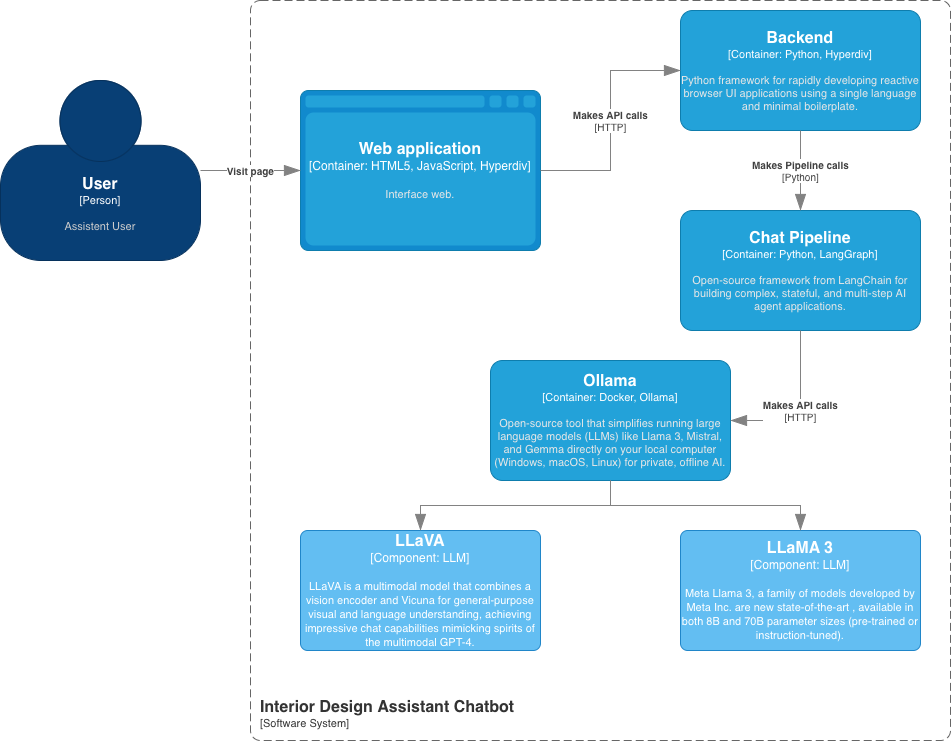
\includegraphics[scale=0.3]{images/c4-system-component.png}
            \caption{Diagrama C4 de Componente.}
         \end{figure}
        
        \subsection{Interface de Utilizador (\textit{Front-end})}
        Foi desenvolvida uma interface web minimalista utilizando a biblioteca Hyperdiv \cite{hyperdiv}. Esta interface foi desenhada para proporcionar uma interação fluida, oferecendo as seguintes funcionalidades:
        
        Gestão de Mensagens: Envio de instruções de texto e visualização do histórico de conversação.
        
        Interação Multimodal: Suporte para anexar ficheiros de imagem, permitindo que o modelo analise o contexto visual do ambiente.
        
        Controlo de Sessão: Opção para limpar o histórico de mensagens e reiniciar o estado da interação.

        \subsection{Arquitetura do \textit{Back-end }e Fluxo de Execução}
        O núcleo da aplicação reside no back-end, onde cada interação do utilizador é processada por um agente inteligente. A lógica de execução é orquestrada através de uma pipeline construída com a biblioteca LangGraph \cite{langgraph}, que permite definir o comportamento do agente como um grafo cíclico de estados.
        
        Ao submeter uma mensagem na interface, os dados são direcionados para o agente, cuja execução está organizada em quatro nós principais:
        \begin{enumerate}
            \item \textbf{Roteador:} Este nó atua como o ponto de entrada da pipeline e é responsável pela triagem dos dados submetidos pelo utilizador. A sua função primordial é verificar a presença de componentes multimodais na mensagem:
            \begin{itemize}
                \item \textbf{Deteção de Imagem:} Caso seja identificado um anexo de imagem, o fluxo é direcionado para o Nó Visual, onde será efetuado o processamento de visão computacional.
                \item \textbf{Fluxo Exclusivamente Textual:} Caso não seja detetada qualquer imagem, o sistema aciona o Nó Textual, otimizando o tempo de resposta ao ignorar as etapas de processamento visual desnecessárias.
            \end{itemize}
            Esta lógica de ramificação garante que o agente utilize o modelo mais adequado para o tipo de dado recebido, assegurando uma gestão eficiente dos recursos computacionais.
            \item \textbf{Textual:} Este nó é ativado sempre que a entrada do utilizador consiste exclusivamente em texto. O processamento é delegado ao modelo LLaMA \cite{llama}, sendo a interação estruturada através de uma instrução de sistema (\textit{System Prompt}) rigorosa que define o comportamento e o domínio de atuação do agente.
            \begin{enumerate}
                \item \textbf{Configuração do Modelo e Diretrizes:} Para garantir a qualidade e a relevância das respostas, o modelo é instanciado com as seguintes diretrizes permanentes:
                \item \textbf{Persona Profissional:} Atuação exclusiva como assistente especializado em Design de Interiores.
                \item \textbf{Estruturação de Respostas:} Obrigatoriedade de fornecer conselhos práticos e profissionais, estruturados preferencialmente em listas ou passos numerados para facilitar a leitura.
                \item \textbf{Foco na Valorização:} Em cenários de potencial venda do imóvel, o modelo é instruído a priorizar intervenções de elevado impacto visual e custo controlado.
                \item \textbf{Localização Linguística:} Tradução e adaptação obrigatória de todos os outputs para português de Portugal.
                \item \textbf{Gestão de Contexto e Memória:} Uma característica fundamental deste nó é a manutenção da coerência conversacional. A cada nova interação, o sistema injeta o histórico completo da sessão atual na pipeline. Esta abordagem permite que o modelo possua memória de curto prazo, sendo capaz de compreender referências a mensagens anteriores e manter a continuidade lógica do diálogo.
            \end{enumerate}
            \item \textbf{Visual:} Este nó é ativado exclusivamente quando o utilizador partilha ficheiros de imagem. A sua função primordial é a transcrição visual, transformando o conteúdo gráfico em dados textuais detalhados que possam ser interpretados pelos nós subsequentes da pipeline.
            Diferente do nó textual, este componente opera de forma isolada no que diz respeito ao histórico de conversação. Para maximizar a velocidade de processamento e reduzir a carga computacional, o histórico de contexto não é enviado. O modelo foca-se estritamente na análise imediata da imagem fornecida, garantindo uma resposta ágil e objetiva.
            O modelo de visão é configurado com uma diretriz específica para assegurar a precisão da análise:
            \begin{itemize}
                \item \textbf{Foco Descritivo:} Atuar como um assistente de design cujo objetivo é listar e descrever todos os elementos visíveis na imagem (mobiliário, iluminação, cores, disposição espacial).
                \item \textbf{Finalidade Técnica:} O output gerado é desenhado para servir de base informativa para o refinamento de sugestões de design que ocorrerá na etapa seguinte.
            \end{itemize}
            A função deste nó não é fornecer o conselho final ao utilizador, mas sim converter a percepção visual em linguagem natural. Este "resumo visual" será posteriormente integrado com o contexto histórico no nó final, garantindo que as sugestões de otimização sejam tecnicamente fundamentadas no que foi efetivamente observado na fotografia.
            \item \textbf{Refinamento:} Este nó constitui a etapa final da pipeline e é ativado sequencialmente após o processamento do Nó Visual. A sua função crítica é a fusão de dados: combinar a descrição técnica da imagem com o histórico da conversação para gerar uma resposta final coerente e personalizada.
            Integração de Dados e Contexto: O diferencial deste nó reside na sua capacidade de contextualização. O sistema injeta a descrição textual gerada anteriormente através da variável \textit{\{image\_description\}}, permitindo que o modelo "compreenda" o que foi visto na imagem sem a necessidade de processar novamente o ficheiro gráfico. O modelo utiliza um conjunto de instruções (\textit{System Prompt}) focado na qualidade do output final:
            \begin{enumerate}
                \item \textbf{Profissionalismo e Clareza:} O foco principal é a melhoria da clareza e do tom profissional dos conselhos de design de interiores.
                \item \textbf{Estruturação Lógica:} Tal como no nó textual, privilegia-se a organização da informação em listas ou passos numerados.
                \item \textbf{Estratégia de Valorização:} Reitera-se a prioridade em mudanças de elevado impacto e custo razoável para objetivos de valorização imobiliária.
                \item \textbf{Finalização Linguística:} Garante que a síntese final entre a análise da imagem e os conselhos teóricos seja entregue integralmente em português de Portugal.
            \end{enumerate}
            Ao consolidar a descrição visual com as intenções do utilizador (presentes no histórico), este nó assegura que as sugestões não são apenas genéricas, mas sim diretamente aplicáveis ao ambiente fotografado. O resultado é uma resposta refinada que encerra o ciclo de processamento do agente.
        \end{enumerate}

        Para uma melhor compreensão da dinâmica de execução e das ramificações de decisão do sistema, apresenta-se a figura \ref{fig:diagrama_fluxo} com o fluxograma do agente de conversação. Este diagrama ilustra a orquestração entre os nós de decisão (roteador), processamento de visão e refinamento textual, evidenciando como o estado é gerido ao longo da pipeline do LangGraph \cite{langgraph}.

        \begin{figure}[!h]
            \centering
            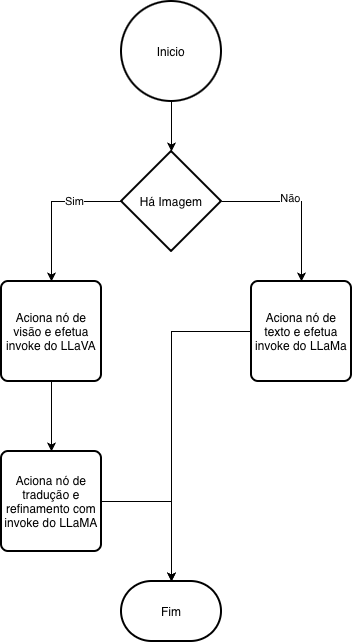
\includegraphics[scale=0.5]{images/diagrama-fluxo.png}
            \caption{Diagrama de Fluxo do Agente do Chat.}
            \label{fig:diagrama_fluxo}
        \end{figure}

        \subsection{Sequenciamento dos Agentes}

        A figura \ref{fig:diagrama_texto} contém o diagrama de sequência  seguinte ilustra o fluxo de execução quando o utilizador submete uma consulta exclusivamente textual. Este processo destaca a natureza síncrona da comunicação e a recuperação do histórico para garantir a continuidade do contexto.

        \begin{figure}[!h]
            \centering
            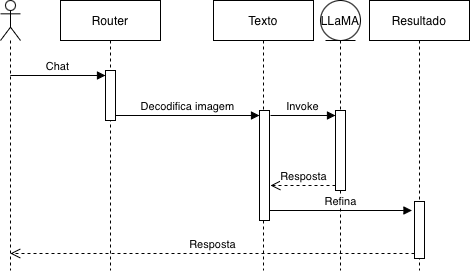
\includegraphics[scale=0.7]{images/diagrama-sequencia-texto.png}
            \caption{Diagrama de Sequencia de acionamento textual.}
            \label{fig:diagrama_texto}
         \end{figure}

        A figura \ref{fig:diagrama_visual} contém fluxo de execução para mensagens que contêm anexos de imagem é mais complexo, exigindo uma orquestração em várias etapas para garantir que o contexto visual seja corretamente interpretado e integrado na resposta final.

        \begin{figure}[!h]
            \centering
            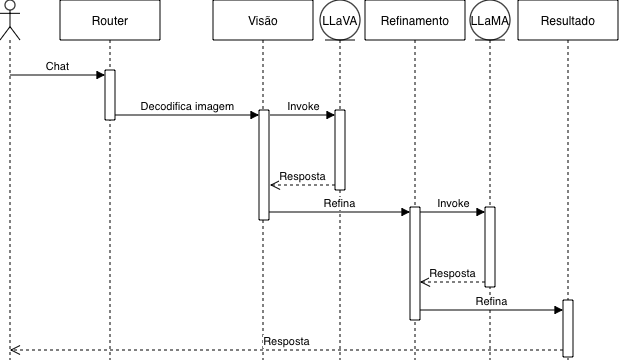
\includegraphics[scale=0.7]{images/diagrama-sequencia-visao.png}
            \caption{Diagrama de Fluxo de acionamento visual.}
            \label{fig:diagrama_visual}
         \end{figure}

         \subsection{Respositório do Código}
         Para efeitos de reprodutibilidade e análise detalhada da implementação, o repositório contendo o código deste trabalho está alojado no GitHub em: https://github.com/diegojeffersonms/IIA

%==========================================================================
% END DESENVOLVIMENTO
%==========================================================================

%==========================================================================
% BEGIN RESULTADOS E AVALIAÇÃO
%==========================================================================

\chapter{Resultados e Avaliação}
    \section{Resultados}
        Os testes realizados demonstraram que o assistente inteligente apresenta um comportamento robusto e alinhado com os objetivos propostos. A análise dos resultados foca-se na eficácia funcional e no desempenho técnico do sistema.

        \begin{figure}[!h]
            \centering
            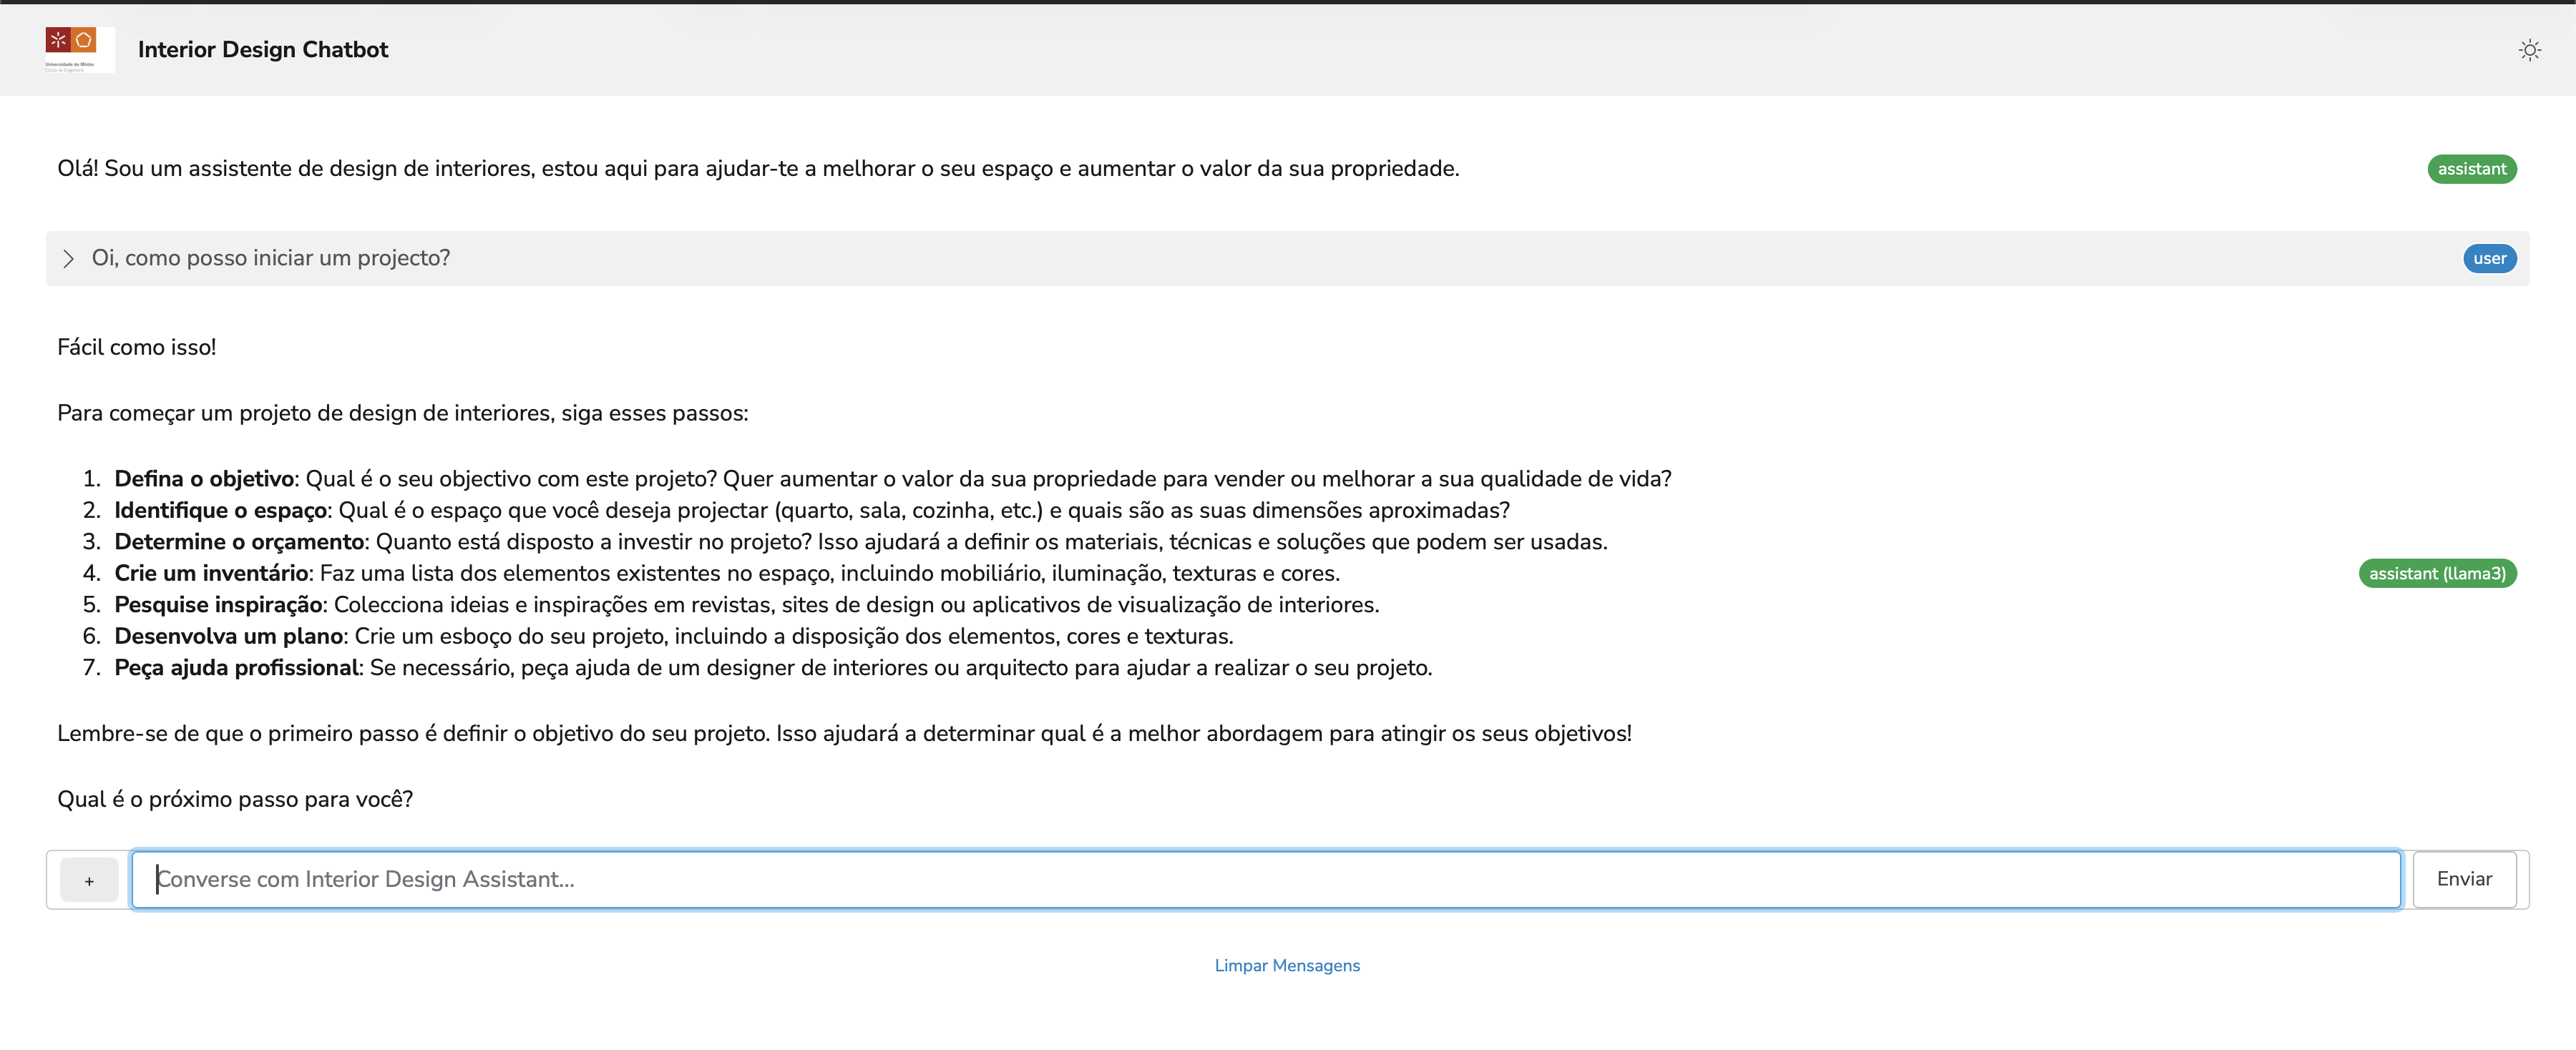
\includegraphics[scale=0.2]{images/chat-textual.png}
            \caption{Uso do Chat com Somente Texto.}
            \label{fig:chat_textual}
        \end{figure}

        \begin{figure}[!h]
            \centering
            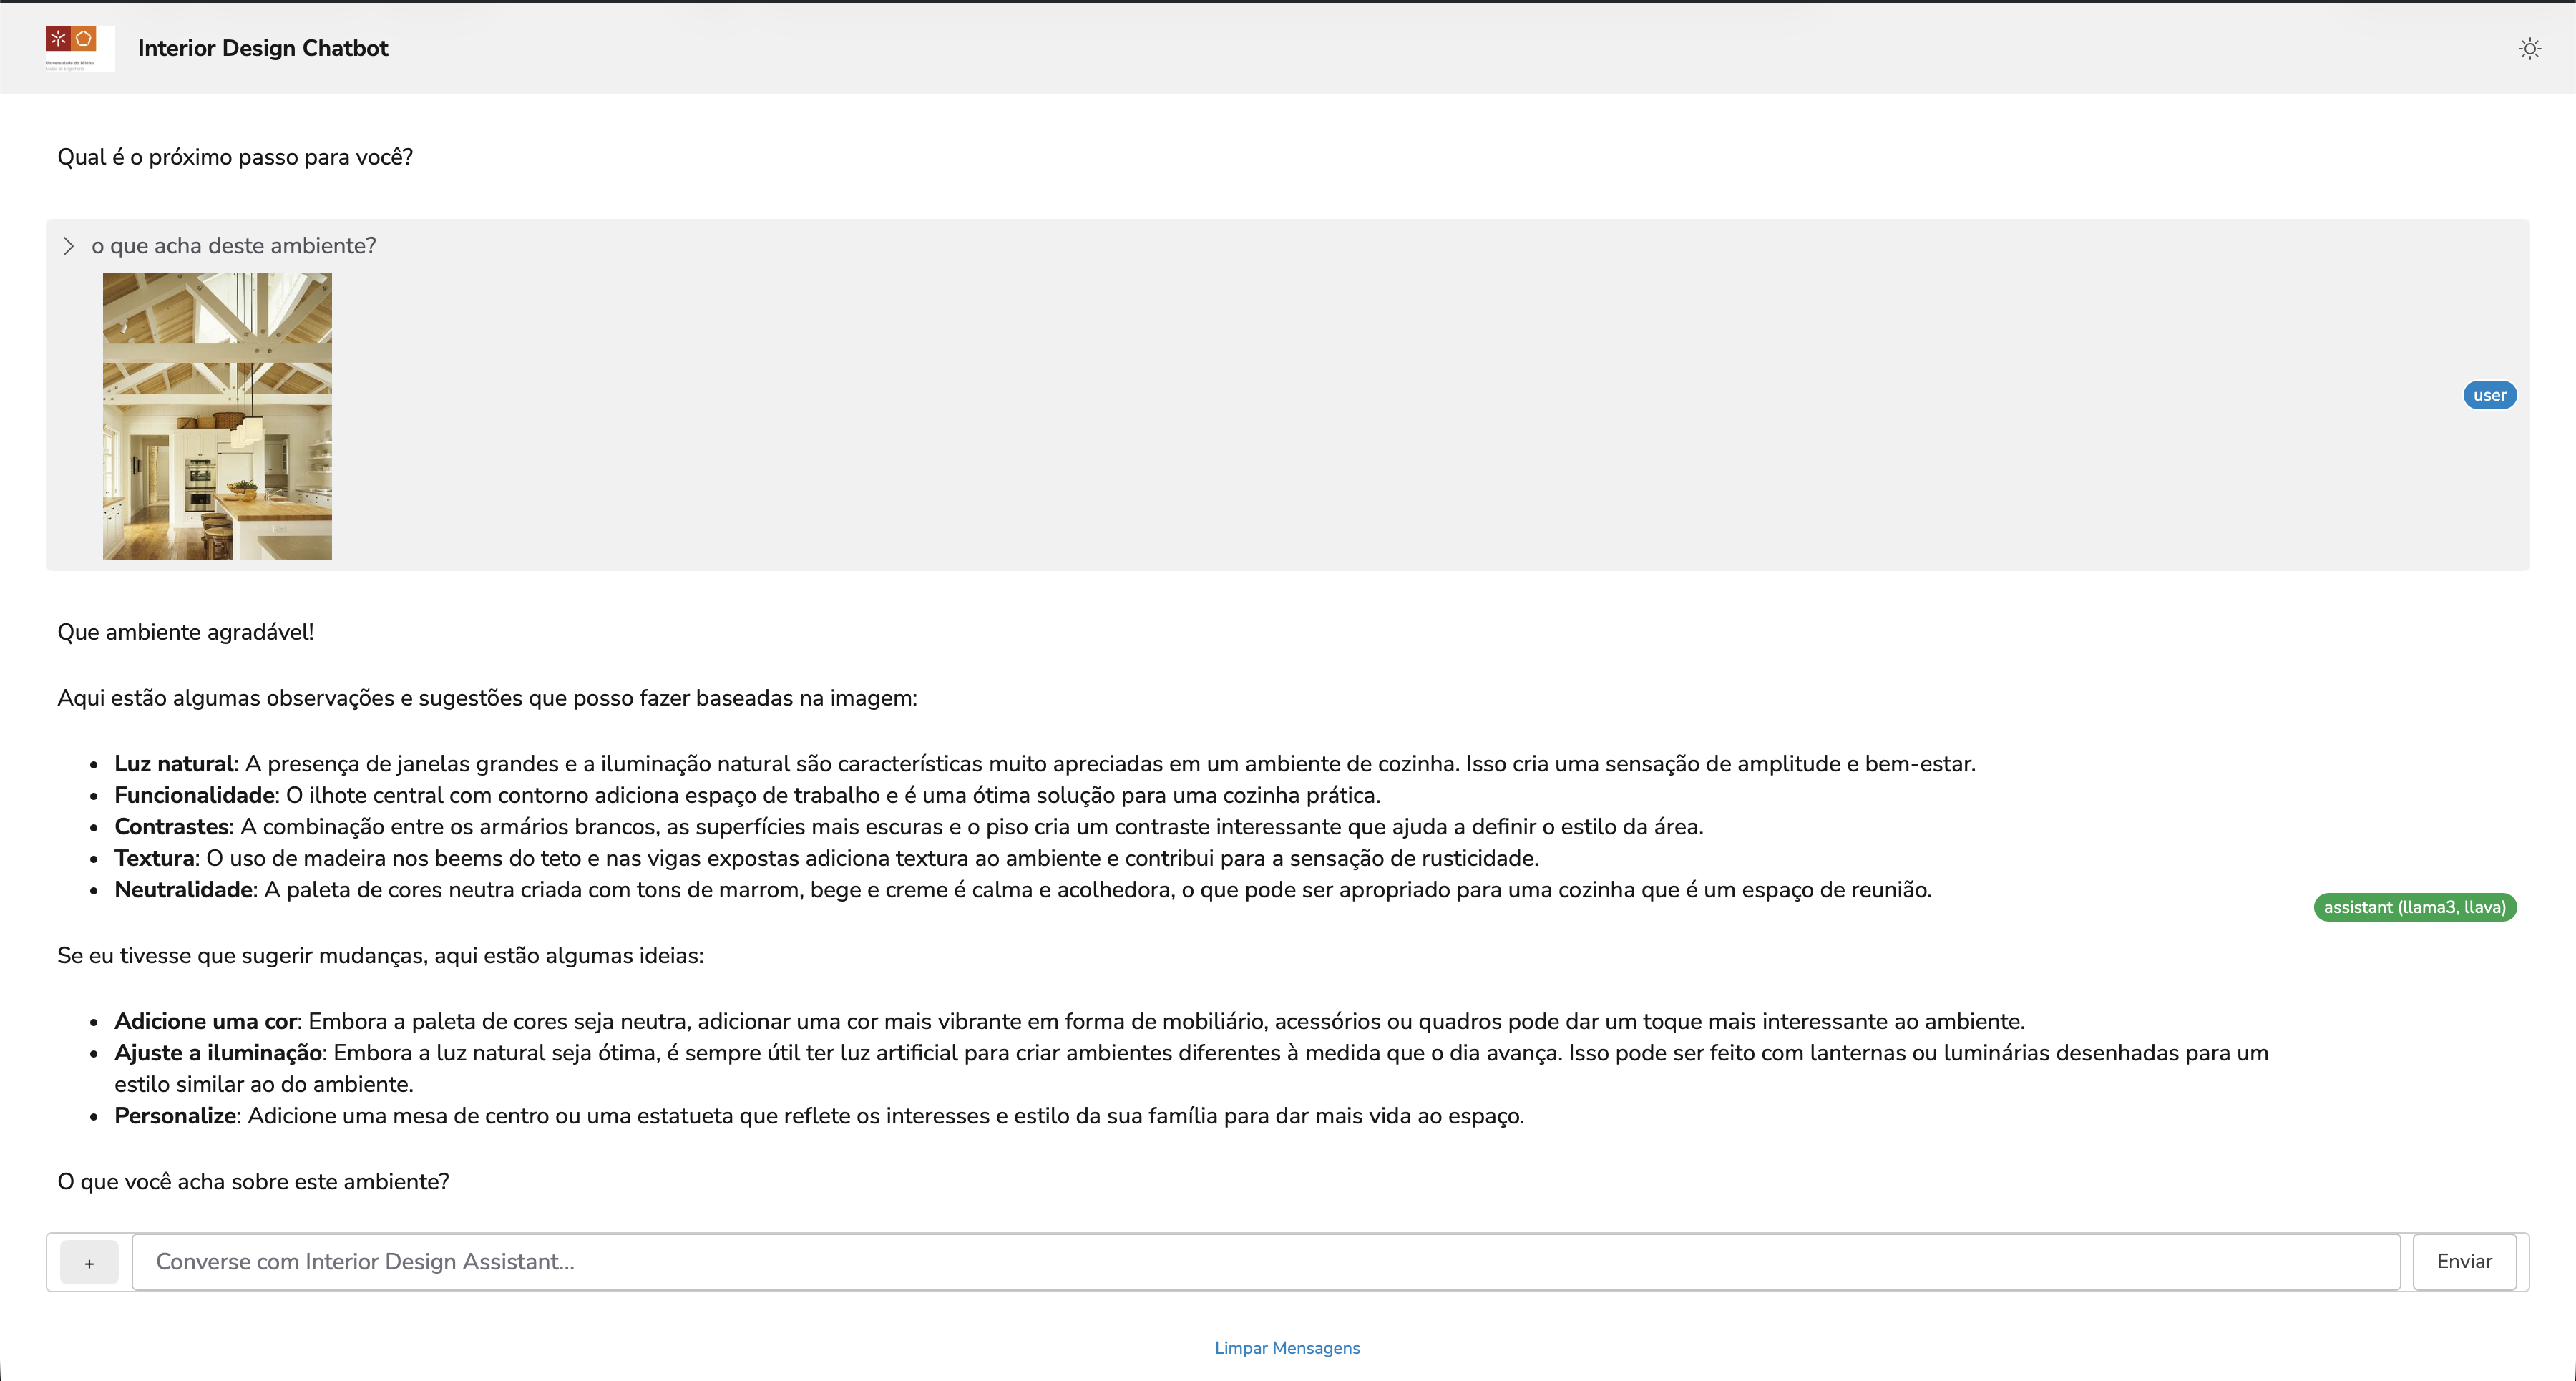
\includegraphics[scale=0.2]{images/chat-visual.png}
            \caption{Uso do Chat com Imagem e Texto.}
            \label{fig:chat_visual}
        \end{figure}

        \subsection{Eficácia Funcional e Qualidade das Respostas}
        O chatbot exibiu uma elevada competência na interpretação de contextos específicos de design de interiores. Observou-se que o sistema foi capaz de:
        \begin{itemize}
            \item \textbf{Interpretação Multimodal:} Identificar corretamente elementos em imagens reais, convertendo-os em descrições textuais úteis para o aconselhamento.
            \item \textbf{Pertinência das Sugestões:} Fornecer recomendações logicamente estruturadas, respeitando as diretrizes de otimização de espaço e valorização imobiliária.
            \item \textbf{Manutenção de Contexto:} Responder adequadamente a sequências de perguntas, demonstrando uma gestão de histórico eficaz durante a sessão.
        \end{itemize}

        \subsection{Desempenho e Viabilidade Técnica}
        Embora o sistema se tenha revelado funcional, o desempenho foi condicionado pela infraestrutura de execução. Devido à utilização do Ollama \cite{ollama} em ambiente Docker \cite{docker} sem aceleração por GPU, registou-se uma latência considerável na geração de respostas. No entanto, este atraso não comprometeu a precisão do modelo, servindo como uma Prova de Conceito para fins acadêmicos bem-sucedido.

        \subsection{Potencial de Evolução}
        Os resultados indicam que a arquitetura baseada em agentes é altamente escalável. Identificou-se que a precisão e a profundidade das respostas podem ser significativamente potenciadas através da implementação de técnicas de RAG (\textit{Retrieval-Augmented Generation}). A integração de uma base de dados vetorial permitiria complementar o conhecimento do modelo com catálogos técnicos, normas de arquitetura ou tendências de mercado atualizadas, reduzindo a ocorrência de alucinações e aumentando a autoridade das sugestões prestadas.

    \section{Discussão Crítica}
        A avaliação do protótipo desenvolvido permitiu identificar pontos fulcrais sobre a aplicação de modelos de linguagem locais em contextos de design de interiores. A análise divide-se entre as competências demonstradas pelo sistema e as condicionantes técnicas inerentes à arquitetura escolhida.

        \subsection{Pontos Fortes e Eficácia do Sistema}
        O sistema demonstrou uma elevada competência na análise multimodal, validando a eficácia da arquitetura em grafos. A capacidade do nó de visão em traduzir elementos espaciais em texto permitiu que o assistente fornecesse conselhos contextuais pertinentes, aproximando-se da percepção humana.
        Ao nível da experiência de utilizador (UX), a implementação de uma interface reativa com suporte para streaming revelou-se crucial. Esta funcionalidade mitiga a percepção de espera, permitindo que o utilizador acompanhe a geração progressiva da resposta. Adicionalmente, o projeto destaca-se pela sua conformidade ética e privacidade. Ao processar todos os dados localmente via Ollama \cite{ollama}, o sistema adere aos princípios de IA Responsável, garantindo que imagens de espaços privados não são transmitidas para servidores de terceiros.

        \subsection{Limitações e Desafios Técnicos}
        Apesar dos resultados positivos, foram identificadas limitações que impactam a escalabilidade da solução:
        \begin{itemize}
            \item Observou-se um tempo de resposta significativo (entre 10 a 30 segundos) no processamento de imagens. Este atraso deve-se à elevada carga computacional exigida pelos modelos de visão em hardware local.
            \item Atualmente, a memória de sessão é volátil. A ausência de uma base de dados dedicada para o histórico de longo prazo implica que o estado da conversação se perca caso a página seja recarregada.
            \item A execução fluida do sistema impõe requisitos técnicos elevados (mínimo de 8GB a 16GB de RAM), o que pode limitar a acessibilidade da ferramenta em dispositivos menos potentes.
        \end{itemize}

        \subsection{Análise Comparativa: Local vs. \textit{Cloud}}
        Comparando esta abordagem com o uso de modelos via API (como o GPT-4o da OpenAI), nota-se um \textit{trade-off} claro. Enquanto uma solução baseada na cloud ofereceria menor latência e uma base de conhecimento mais vasta, comprometeria a soberania de dados e a privacidade das imagens dos utilizadores, além de introduzir custos variáveis por utilização. O modelo local adotado neste trabalho posiciona-se como uma "caixa-preta" segura e privada, priorizando a segurança em detrimento da velocidade instantânea.

%==========================================================================
% END RESULTADOS E AVALIAÇÃO
%==========================================================================

%==========================================================================
% BEGIN CONCLUSÕES DE TRABALHO FUTURO
%==========================================================================

\chapter{Conclusões e Trabalho Futuro}
    O presente trabalho permitiu demonstrar a viabilidade e o potencial da aplicação de Inteligência Artificial Generativa na democratização do acesso a serviços de design de interiores e otimização habitacional. Através do desenvolvimento de um agente inteligente multimodal, foi possível responder à crescente necessidade de maximização de espaços em contextos urbanos de elevada densidade.
    A arquitetura implementada, baseada na orquestração de grafos de estado com o LangGraph \cite{langgraph} e na execução local de modelos via Ollama \cite{ollama}, revelou-se uma escolha técnica sólida. Esta abordagem não só garantiu a flexibilidade necessária para gerir fluxos complexos (texto e imagem), como também assegurou a total privacidade e soberania dos dados dos utilizadores, um fator crítico quando se lida com registos visuais de ambientes privados.
    Apesar das limitações identificadas ao nível da latência — decorrentes da execução em hardware sem aceleração dedicada (GPU) — o projeto atingiu com sucesso o estatuto de Prova de Conceito (PoC). O ChatBot demonstrou uma capacidade notável de interpretação visual e raciocínio lógico, fornecendo sugestões pertinentes e personalizadas que cumprem o objetivo de valorização funcional e patrimonial dos imóveis.
    
    \subsection{Trabalhos Futuros}
    Como perspetiva de evolução, este projeto estabelece os alicerces para implementações mais sofisticadas. Sugere-se para investigações futuras:
    \begin{itemize}
        \item Implementação de RAG (Retrieval-Augmented Generation) com uso de bases de dados externas para garantir que o assistente utiliza conhecimentos técnicos e normativas arquitetónicas atualizadas.
        \item Persistência de Longo Prazo com desenvolvimento de uma camada de base de dados para manter o histórico entre sessões, permitindo um acompanhamento contínuo de projetos de renovação.
    \end{itemize}
    Em suma, este trabalho evidencia que a IA, quando estruturada de forma modular e ética, pode atuar como uma ferramenta poderosa de apoio à decisão, transformando desafios demográficos e imobiliários em oportunidades de inovação tecnológica.

%==========================================================================
% END CONCLUSÕES DE TRABALHO FUTURO
%==========================================================================

%==========================================================================
% BEGIN REFERÊNCIAS
%==========================================================================

%% Changes biblibography name
%% Portuguese babel default : "Bibliografia"
%% Personally I prefer "Referências"
\renewcommand\bibname{Referências}

%% https://www.overleaf.com/learn/latex/bibliography_management_with_bibtex
\begin{thebibliography}{9}
\bibitem{ollama}
OLLAMA (2024). Ollama: Get up and running with large language models. [Online]. Disponível em: https://ollama.com [Acedido em: 11 de janeiro de 2026].
\bibitem{llava}
YOUNG, H. et al. (2023). LLaVA: Large Language and Vision Assistant. [Online]. Disponível em: https://llava-vl.github.io [Acedido em: 11 de janeiro de 2026].
\bibitem{llama}
META AI (2024). Introducing Llama 3: The most capable openly available LLM to date. [Online]. Disponível em: https://ai.meta.com/blog/meta-llama-3/ [Acedido em: 11 de janeiro de 2026].
\bibitem{langgraph}
LANGCHAIN (2024). LangGraph: Building Language Agents with Graphs. [Online]. Disponível em: https://www.langchain.com/langgraph [Acedido em: 11 de janeiro de 2026].
\bibitem{hyperdiv}
STEFANOVIC, M. (2024). Hyperdiv: Reactive web UI framework for Python. [Online]. Disponível em: https://hyperdiv.io [Acedido em: 11 de janeiro de 2026].
\bibitem{docker}
DOCKER (2024). Docker Documentation. [Online]. Disponível em: https://docs.docker.com [Acedido em: 11 de janeiro de 2026].
\end{thebibliography}

%==========================================================================
% END REFERÊNCIAS
%==========================================================================

%==========================================================================
% BEGIN LISTA DE SIGLAS E ACRÓNIMOS
%==========================================================================

%% Portuguese babel does not translate this environment
\renewcommand{\nomname}{Lista de Siglas e Acrónimos}

%% acronyms
\nomenclature[01]{\textbf{IA}}{Inteligência Artificial}
\nomenclature[02]{\textbf{LLM}}{\textit{Large Language Model} - Modelo de Linguagem Grande}
\nomenclature[03]{\textbf{LLaMA}}{Modelo de linguagem de texto da Meta}
\nomenclature[04]{\textbf{LLaVA}}{\textit{Large Language and Vision Assistant} - Modelo multimodal}
\nomenclature[05]{\textbf{GPU}}{\textit{Graphic Process Unit} - Unidade de Processamento Gráfico}
\nomenclature[06]{\textbf{PoC}}{\textit{Proof of Concept} - Prova de Conceito}
\nomenclature[07]{\textbf{RAG}}{\textit{Retrieval-Augmented Generation} - Geração Aumentada via Recuperação}
\nomenclature[08]{\textbf{API}}{\textit{Application Programming Interface} - Interface de Programação de Aplicação}
\nomenclature[09]{\textbf{RAM}}{\textit{Random Access Memory} - Memória de Acesso Aleatório (ou Randómico)}
\nomenclature[10]{\textbf{GB}}{\textit{Gigabyte} - uma unidade de medida de armazenamento ou memória}
\nomenclature[11]{\textbf{UX}}{\textit{User Experience} - Experiência do Usuário}
\nomenclature[12]{\textbf{TF-IDF}}{\textit{Term Frequency–Inverse Document Frequency} - Frequência do Termo–Inverso da Frequência}
\nomenclature[13]{\textbf{QA}}{\textit{Quality Assurance} - Garantia de Qualidade}

%% Show acronyms
\printnomenclature

%==========================================================================
% END LISTA DE SIGLAS E ACRÓNIMOS
%==========================================================================

%==========================================================================
% BEGIN ANEXOS
%==========================================================================

%% Why \addchap, instead of \chapter? 
%% \addchap has no numbering but appears in table of contents.
%% \addchap{Anexos}

%%     <<Os anexos deverão ser utilizados para a inclusão de informação adicional necessária para uma melhor compreensão do relatório o para complementar tópicos, secções ou assuntos abordados. Os anexos criados deverão ser numerados e possuir uma designação. Estes dados permitirão complementar o Índice geral do relatório relativamente à enumeração e apresentação dos diversos anexos.>>
    
    %% section version of \addchap
%%     \addsec{Anexo 1}


%==========================================================================
% END ANEXOS
%==========================================================================
\end{document}